\section*{Lucrarea de laborator \#2}
\phantomsection

\section{Scopul lucrarii de laborator :}
Realizeaza un simplu GUI Calculator care suporta operatiile simple de +, -, *, /, putere, radical, InversareSemn(+/-), operatii cu numere zecimale.

\section{Obiective si Conditii Necesare :}
Familiarizarea cu un nou limbaj de programare, si folosirea unui nou IDE, pentru dezvoltarea cunostintelor noastre in limbaje si medii interactive de dezvoltare a programelor.

\section{Mersul lucrarii :}
In aceasta lucrare am elaborat un Calculator , care e friendly pentru utilizator. 

\textbf{Note si explicatii !}
\subsection{Partea Grafica}
\tab Cind am creat fereastra, implicit are o denumire pe care o vom modifica corespunzator in Calculator din menu-l \textbf{Properties}, modificam cimpul \textbf{Text}. \\
\\
Pentru a nu schimba dimensiunea ferestrei , si a avea dimensiunea stabilita de noi vom dezactiva optiunea de \textbf{Maximize} si \textbf{Restore Down} din menu-l \textbf{Properties}, modificam valoarea cimpului MaximizeBox din True in False , si 
cimpul \textbf{FormBorderStyle} il modificam din \textbf{Sizable} in \textbf{FixedSingle}. \\
\\
Pentru a adauga butoane pe forma , din \textbf{ToolBox} selectam \textbf{Button, TextBox} si \textbf{Label} ca componente vizuale caruia din \textbf{Properties} ii putem modifica orice proprietate,cum ar fi : marimea, font-ul, numele, etc. Analog adaugam un TextBox pentru afisarea rezultatului. \\
\\
Pentru fiecare buton am scris codul, adica functionalitatea 
acestuia.Astfel,in continuare, voi explica momentele principale si importante de stiut.\\

\subsection{Modulul de baza}
\textbf{ Butonul CE (Clear Entry) / C (Clear all)} \\
Functionalitatea acestuia consta in faptul ca cifra/cifrele introduse se sterg si "se transforma" in 0: \\
 \textbf{ txtDisplay.Text = "0";} \\
Adica la tastarea butonului \textbf{CE} , proprietatea Text a componentei vizuale TextBox, denumita de mine txtDisplay va lua valoarea 0, exact acelasi rezultat va fi si la tastarea 
butonului \textbf{C}. \\
\begin{figure}[h]
\centering
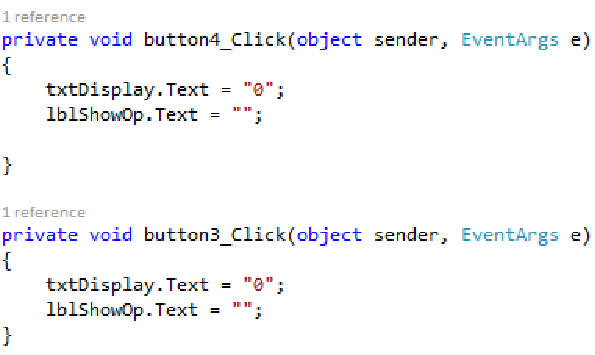
\includegraphics[scale=1]{1.pdf}
\end{figure}
\cleardoublepage
\textbf{Butonul Backspace} \\
Functionalitatea acestuia consta in faptul ca la tastarea lui, ultima cifra introdusa va fi stearsa. Pentru asta am folosit 2 cicluri : primul if verifica lungimea stringului ( pentru ca propietatea \textbf{Text} a TextBox-ului este de tip \textbf{String}) este mai mare ca 0 (adica putem ceva sterge), atunci din lungimea 
sirului de cifre, se sterge ultimul caracter : \\
\textbf{txtDisplay.Text = 
txtDisplay.Text.Remove(txtDisplay.Text.Length - 1);}\\
Si al doilea if, verifica daca proprietatea Text a TextBox-ului are un string null, atunci la tastarea butonului Backspace, valoarea va fi setata cu 0.\\
\begin{figure}[h]
\centering
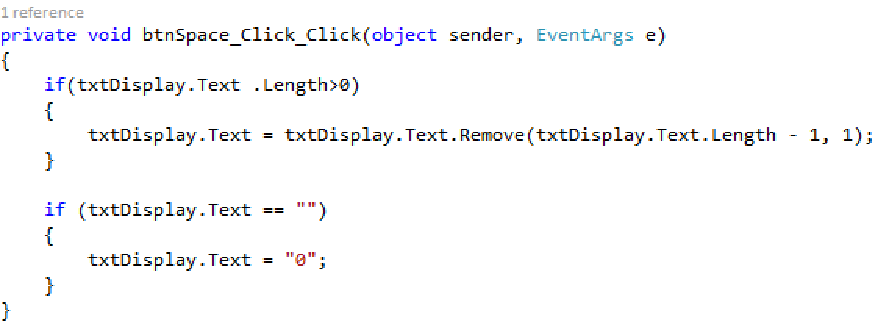
\includegraphics[scale=1]{2.pdf}
\end{figure}
\cleardoublepage

\textbf{Operatorii aritmetici } \\
Cind vom tasta pe unul din operatorii + , - , / , * atunci se va apela metoda ce urmeaza sa o descriu.Deci, am creat o variabila de tip Button in care se stocheaza butonul ce vine. Orice operator tastat el vine in aceasta functie, iar variabila \textbf{num} preia butonul cu toate caracteristicile lui,iar variabila operation preia semnul prin \textbf{num.Text;}
\begin{figure}[h]
\centering
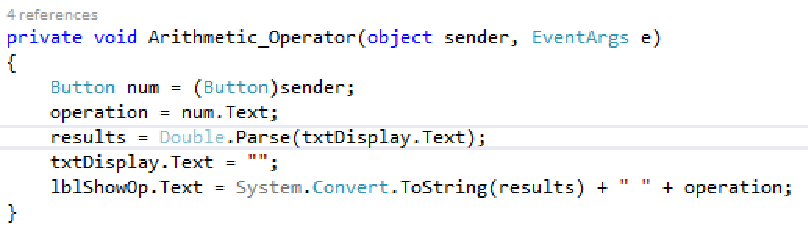
\includegraphics[scale=1]{3.pdf}
\end{figure}

\textbf{Butonul Egal } \\
In aceasta metoda,am folosit o instructiune de selectie Switch, care in dependenta de operatorul ales, el va alege cazul corespunzator. Voi explica codul pentru un operator, pentru ca analogic este codul si pentru ceilalti operatori: \\
\textbf{case "+": \\
\tab \tab txtDisplay.Text = (results + Double.Parse(txtDisplay.Text)) .ToString();\\
\tab break;}\\
Continutul proprietatii Text ai componentei vizuale txtDisplay (TextBox), va fi parsat in tipul de date Double, pentru a putea si adaugat cu valoarea lui results , care a fost initializata cu 0. Am obtinut un rezultat concret, un numar. Acest numar , cu ajutorul metodei ToString este convertita intr-un String, pentru ca proprietatea Text a Textbox-ului asteapta un String, daca primeste alt tip de date, atunci vom avea eroare. Respectiv se face break - care este iesirea conditionata din instructiune, celelalte case-uri fiind ignorate. 
\begin{figure}[h]
\centering
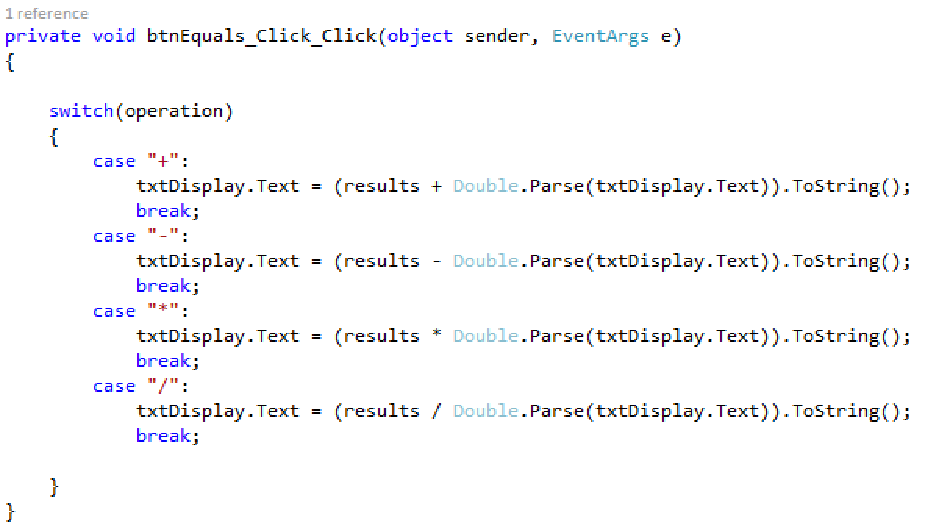
\includegraphics[scale=1]{4.pdf}
\end{figure}
\clearpage

\textbf{Butonul Sqrt} \\
Am declarat o variabila de tip Double, careia i-am atribuit valoarea preluata din txtDisplay si parsata in Double, respectiv acestei variabile locale, i-am atribuit rezultatul unei functii  , si anume Math.Sqrt(), care primeste ca parametru insasi valoarea preluata din txtDisplay. Respectiv rezultatul final, va fi parsat cu ToString si atribuit proprietatii text: \\
\textbf{txtDisplay.Text = System.Convert.ToString(sq);} \\

\begin{figure}[h]
\centering
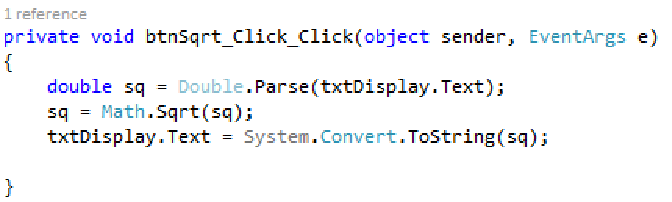
\includegraphics[scale=1]{5.pdf}
\end{figure}

\textbf{ Butonul +/- } \\
In aceasta metoda am declarat o variabila careia i-am atribuit valoarea din txtDisplay convertita in ToDouble. In continuare  a = a*(-1); si valoarea obtinuta am convertit-o in ToString, si atribuit-o Text-ului: \\
\textbf{txtDisplay.Text = System.Convert.ToString(a);}
\begin{figure}[h]
\centering
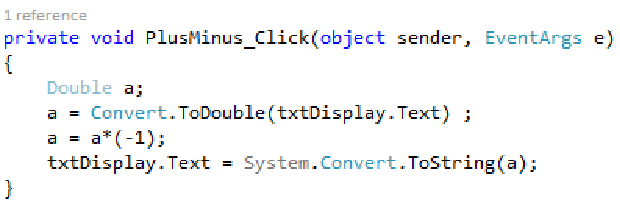
\includegraphics[scale=1]{6.pdf}
\end{figure}
\clearpage
\section{Screenshoot-uri}
\begin{figure}[h]
\centering
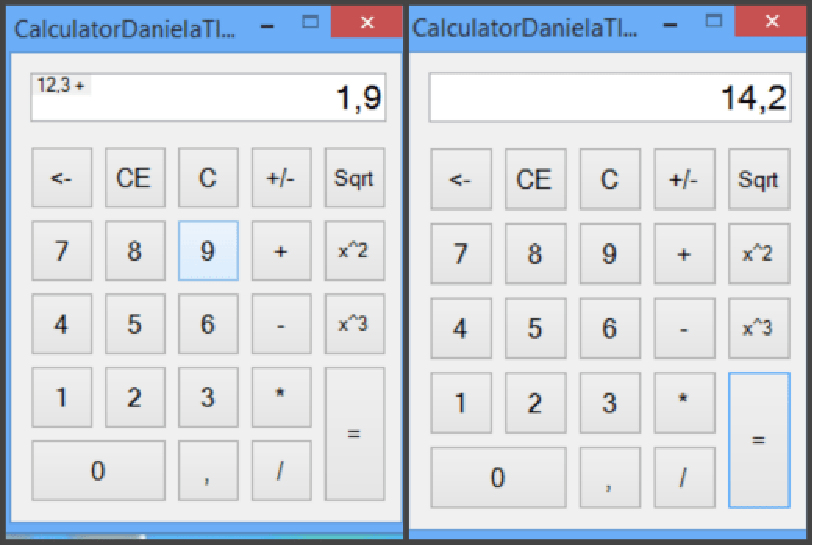
\includegraphics[scale=1]{image.pdf}
\end{figure}

\begin{figure}[h]
\centering
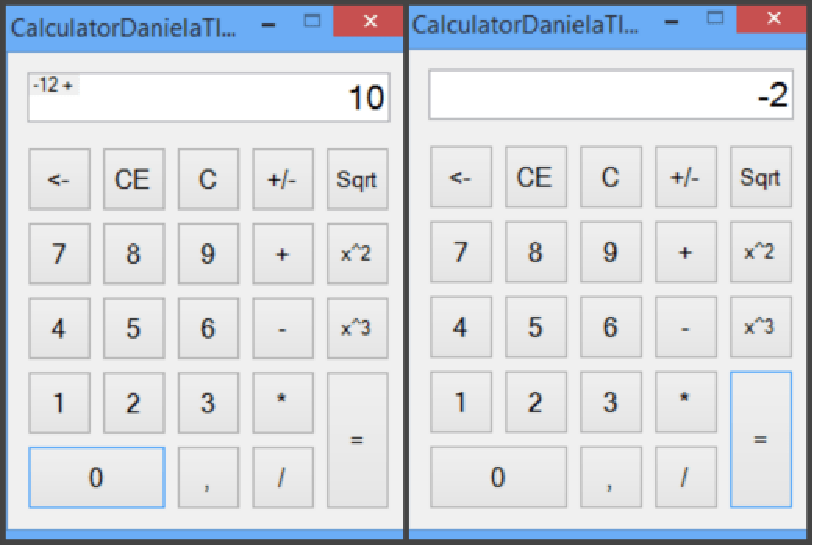
\includegraphics[scale=1]{colaj2.pdf}
\end{figure}

\clearpage
\section{Concluzii}

\tab In acest laborator, am facut cunostinta cu ceva total nou pentru mine, limbajul C-Sharp.Mi-a placut,e usor de utilizat,contine functii care m-au ajutat mult precum \textbf{Parse , ToString, ToDouble} si proprietati precum \textbf{.Text , .Remove , .Lenght , .Contains}.Pentru un limbaj de nivel inalt este foarte okey sa poti interactiona cu limbajul friendly. De asemenea si IDE-ul folosit (\textbf{Visual Studio}) este comod, este bine aranjat cu menu-uri,care ulterior pot fi rearanjate dupa comoditate.Totusi, bazindu-ma mai mult tehnic, calculatorul a avut nevoie de cunostinte bune si nunate de stiut, m-am documentat pe Internet, am folosit surse,tutoriale din \textbf{Youtube}, care m-au ajutat mult sa realizez aceasta lucrare.
\clearpage